\section{Ziele der Arbeit}
\label{chap:goals}


Das Ziel dieser Diplomarbeit ist es, die zeitliche Veränderung von Themen in Textsequenzen zu erfassen. Im Speziellen soll die Prominenz der Themen erfasst und die Veränderungen über die Zeit dargestellt werden. Ein Thema ist ein prominentes Thema, wenn es oft in einer Textsequenz auftritt. Es könnten nun, wie in es in \citet{ldaSourceCode} angewendet wird, für jeden Zeitabschnitt die Themen gelernt werden und gezählt werden, wie oft ein Thema vorkommt. Dieser Ansatz ist jedoch für die vorliegende Arbeit ungeeignet, da erstens die Ergebnisse als Online-Algorithmus im SCY-Projekt benutzt werden sollen und das Lernen der Themen doch eine zeitaufwändige Aufgabe ist. Zweitens werden hier die Wahrscheinlichkeiten des Auftretens der Themen nicht berücksichtigt, sondern es wird jedes Auftreten gezählt.

Der Ansatz in dieser Arbeit ist ähnlich, in wichtigen Punkten unterscheidet er sich jedoch. Zum einen wird zwischen der Lernphase und der Anwendungsphase unterschieden. In der Lernphase wird anhand von Hintergrundtexten ein Themenmodell trainiert. Diese Hintergrundtexte sind nicht notwendigerweise zeitlich sortiert und enthalten Informationen über die Themen, die trainiert werden sollen. Dies sind zum Beispiel Artikel der Deutschen Presse Agentur (dpa) zu bestimmten Themen wie Politik, Kunst oder, im Kontext des SCY-Projektes, Texte mit Hintergrundwissen für die aktuelle zu bearbeitende Mission. So kann ein Themenmodell erstellt werden, das für den speziellen Kontext geeignet ist. Diese Eignung soll in der Diplomarbeit auch validiert werden. Die genaue Vorgehensweise wird in Kapitel \ref{chap:workflowData} behandelt. Die Qualität der Themenmodelle hängt direkt von der Vorverarbeitung der Texte ab. Es muss also zusätzlich ermittelt werden, welche Vorverarbeitunsschritte die Qualität der Themenmodelle beeinflussen.

\begin{figure}[ht]
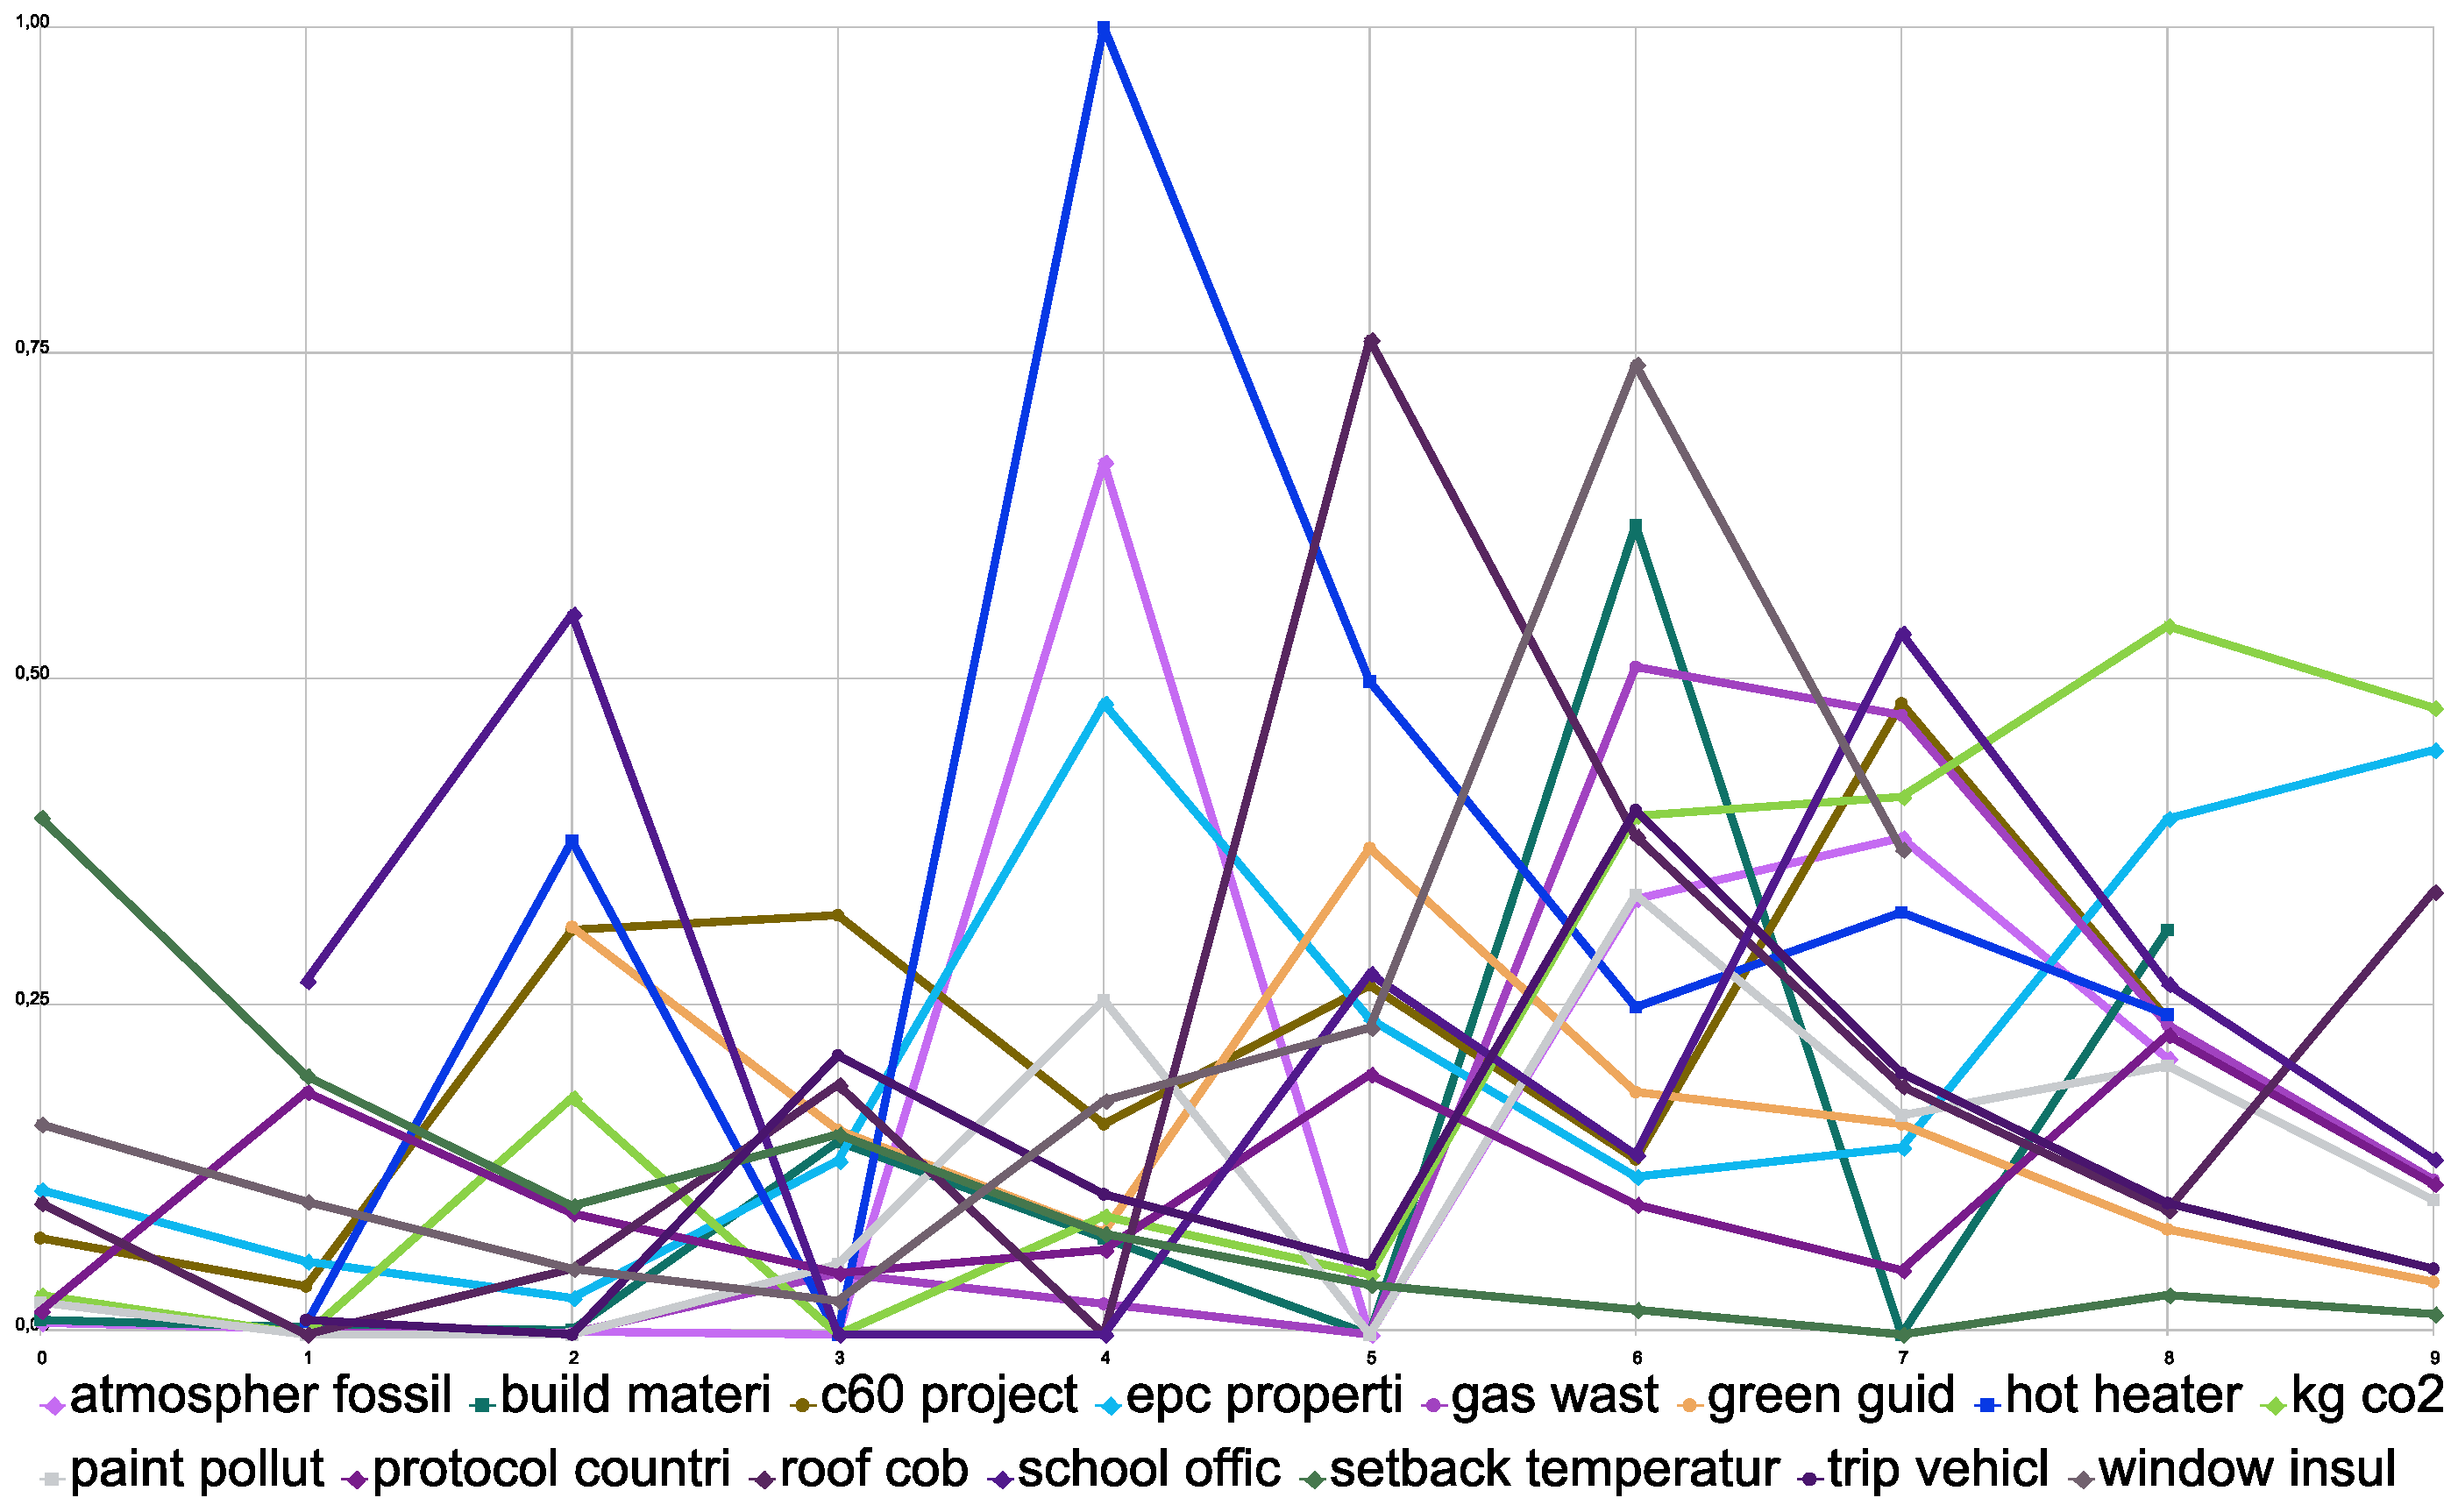
\includegraphics[width=1.0\textwidth]{images/content/01_introduction/chart_betweeness} 
\caption{Visualisierung der Themenveränderung}
\label{fig:topicChange}
\end{figure}

In der Anwendungsphase werden die vorkommenden Themen identifiziert, deren Wichtigkeit bewertet und schlussendlich die zeitliche Verände"-rung dargestellt. Dazu werden, wie in \citet{shafferEpistemicFrames}, die Textsequenzen in diskrete zeitliche Abschnitte unterteilt. Die Einteilung richtet sich dabei nach vorhandenen Dokumenten. In einen zeitlichen Abschnitt werden eine bestimmte Anzahl von zeitlich aufeinander folgenden Dokumenten zusammengefasst. Je nach Größe der Zeitabschnitte können so verschieden Zeiträume betrachtet werden. Im Falle von Chatnachrichten kann ein Zeitabschnitt nur ein paar Minuten umfassen, während im Falle von Nachrichten die Zeitabschnitte eine Woche, einen Monat oder mehr abdecken können. Da die Wahl der Größe der Zeitabschnitte unabhängig vom gelernten Themenmodell ist, können so auch verschiedene Zeiträume in annehmbarer Zeit betrachtet und verglichen werden. 

Für jedes Dokument in einem Zeitabschnitt werden die vorkommenden Themen und die Wahrscheinlichkeit, mit der diese Themen vorkommen, ermittelt. Aus den ermittelten Themen wird anhand der Kookkurrenz und den Wahrscheinlichkeiten eine Graphenstruktur aufgebaut. Es werden verschiedene Algorithmen entwickelt, die dann auf ihre Eignung geprüft werden. Auf die Graphen werden dann verschiedene Zentralitätsindizes angewendet. Zentralitätsindizes bewerten die Wichtigkeit eines Knoten in einem Graphen. So wird die Prominenz der Themen ermittelt. Auch hier gilt es zu evaluieren, welcher Zentralitätsindex am besten geeignet ist, die Prominenz der Themen zu bewerten. 

Wenn mehrere Zeitabschnitte nacheinander betrachtet werden, kann die thematische Verände"-rung einfach visualisiert werden. Hierzu werden die Veränderungen als Kurve dargestellt. In Abbildung \ref{fig:topicChange} ist ein Beispiel für eine solche Visualisierung dargestellt. Da die Visualisierung unübersichtlich werden kann, wenn viele Themen auftreten, werden auch hier verschiedene Ansätze untersucht.

Es gilt also folgende Probleme zu lösen: 
\begin{itemize} 
  \item Themenmodelle anhand von Hintergrundtexten zu trainieren und ihre Eignung für die Aufgabenstellung zu evaluieren.
  \item Textsequenzen in diskrete Zeitabschnitte zu unterteilen und festzustellen, welche Größe der Zeitabschnitte für die verschiedenen Textdatensätze geeignet ist.
  \item Aus den ermittelten Themen einen Graphen zu erstellen und zu prüfen, welcher Algorithmus zusammen mit den Zentralitätsindizes die zugrundeliegenden Themen in den Texten am besten repräsentiert.
  \item eine geeignet Art der Visualisierung entwickeln.
\end{itemize} 
